\chapter{基礎データ}
\label{付録}

\section{EMNIST Digitsデータセットの基礎データ}
\begin{figure}[H]
    \centering
    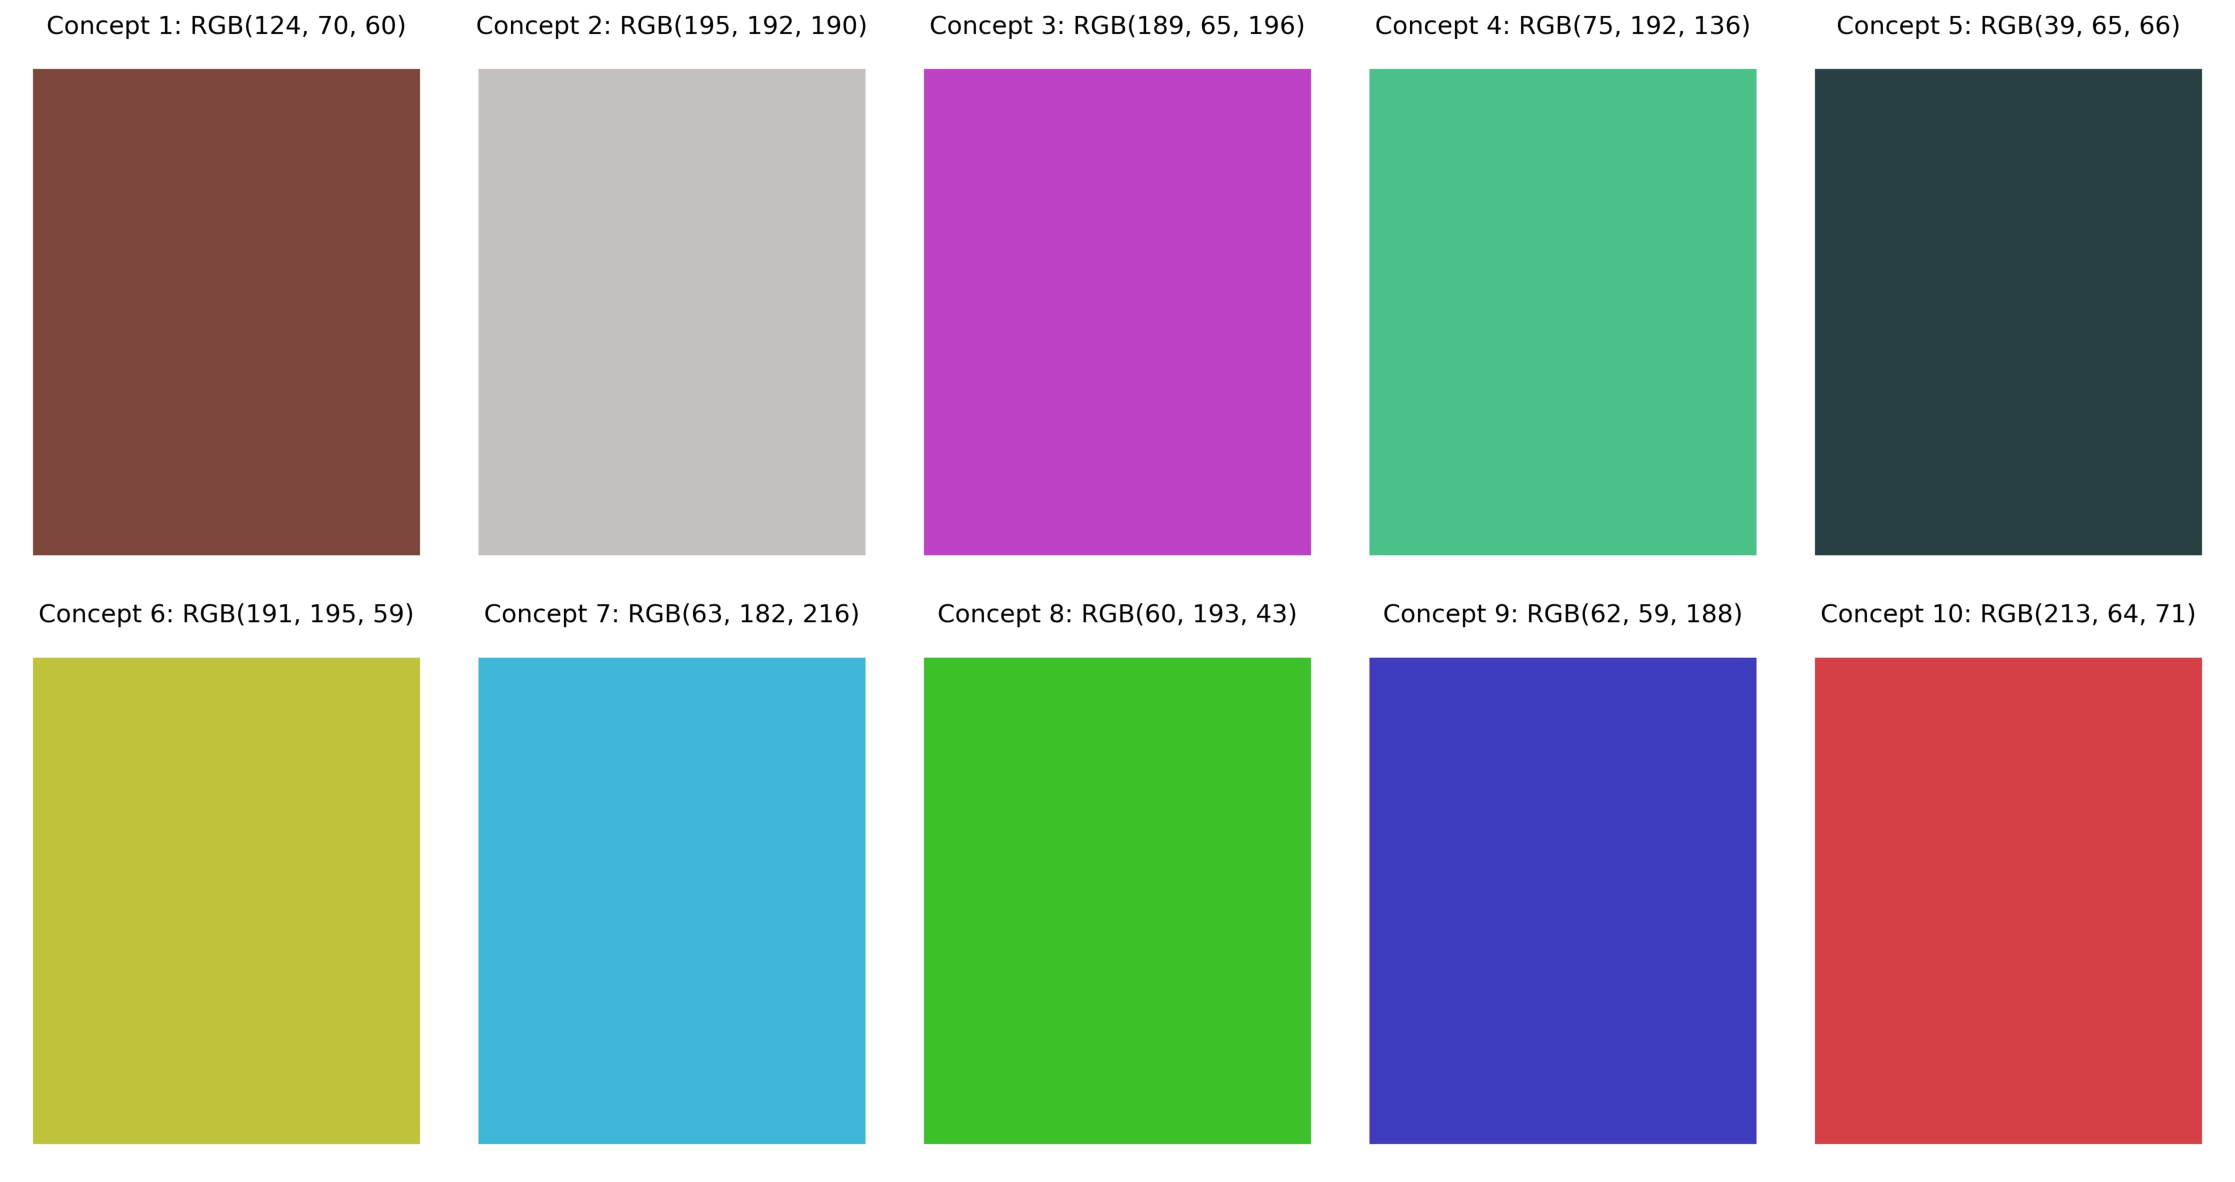
\includegraphics[width=\linewidth]{fig/color_varinace/0.pdf}
    \caption{$\sigma^2 = 0.0$の場合の各色クラスの色の例}
    \label{fig:variance_0}
\end{figure}

\begin{figure}[H]
    \centering
    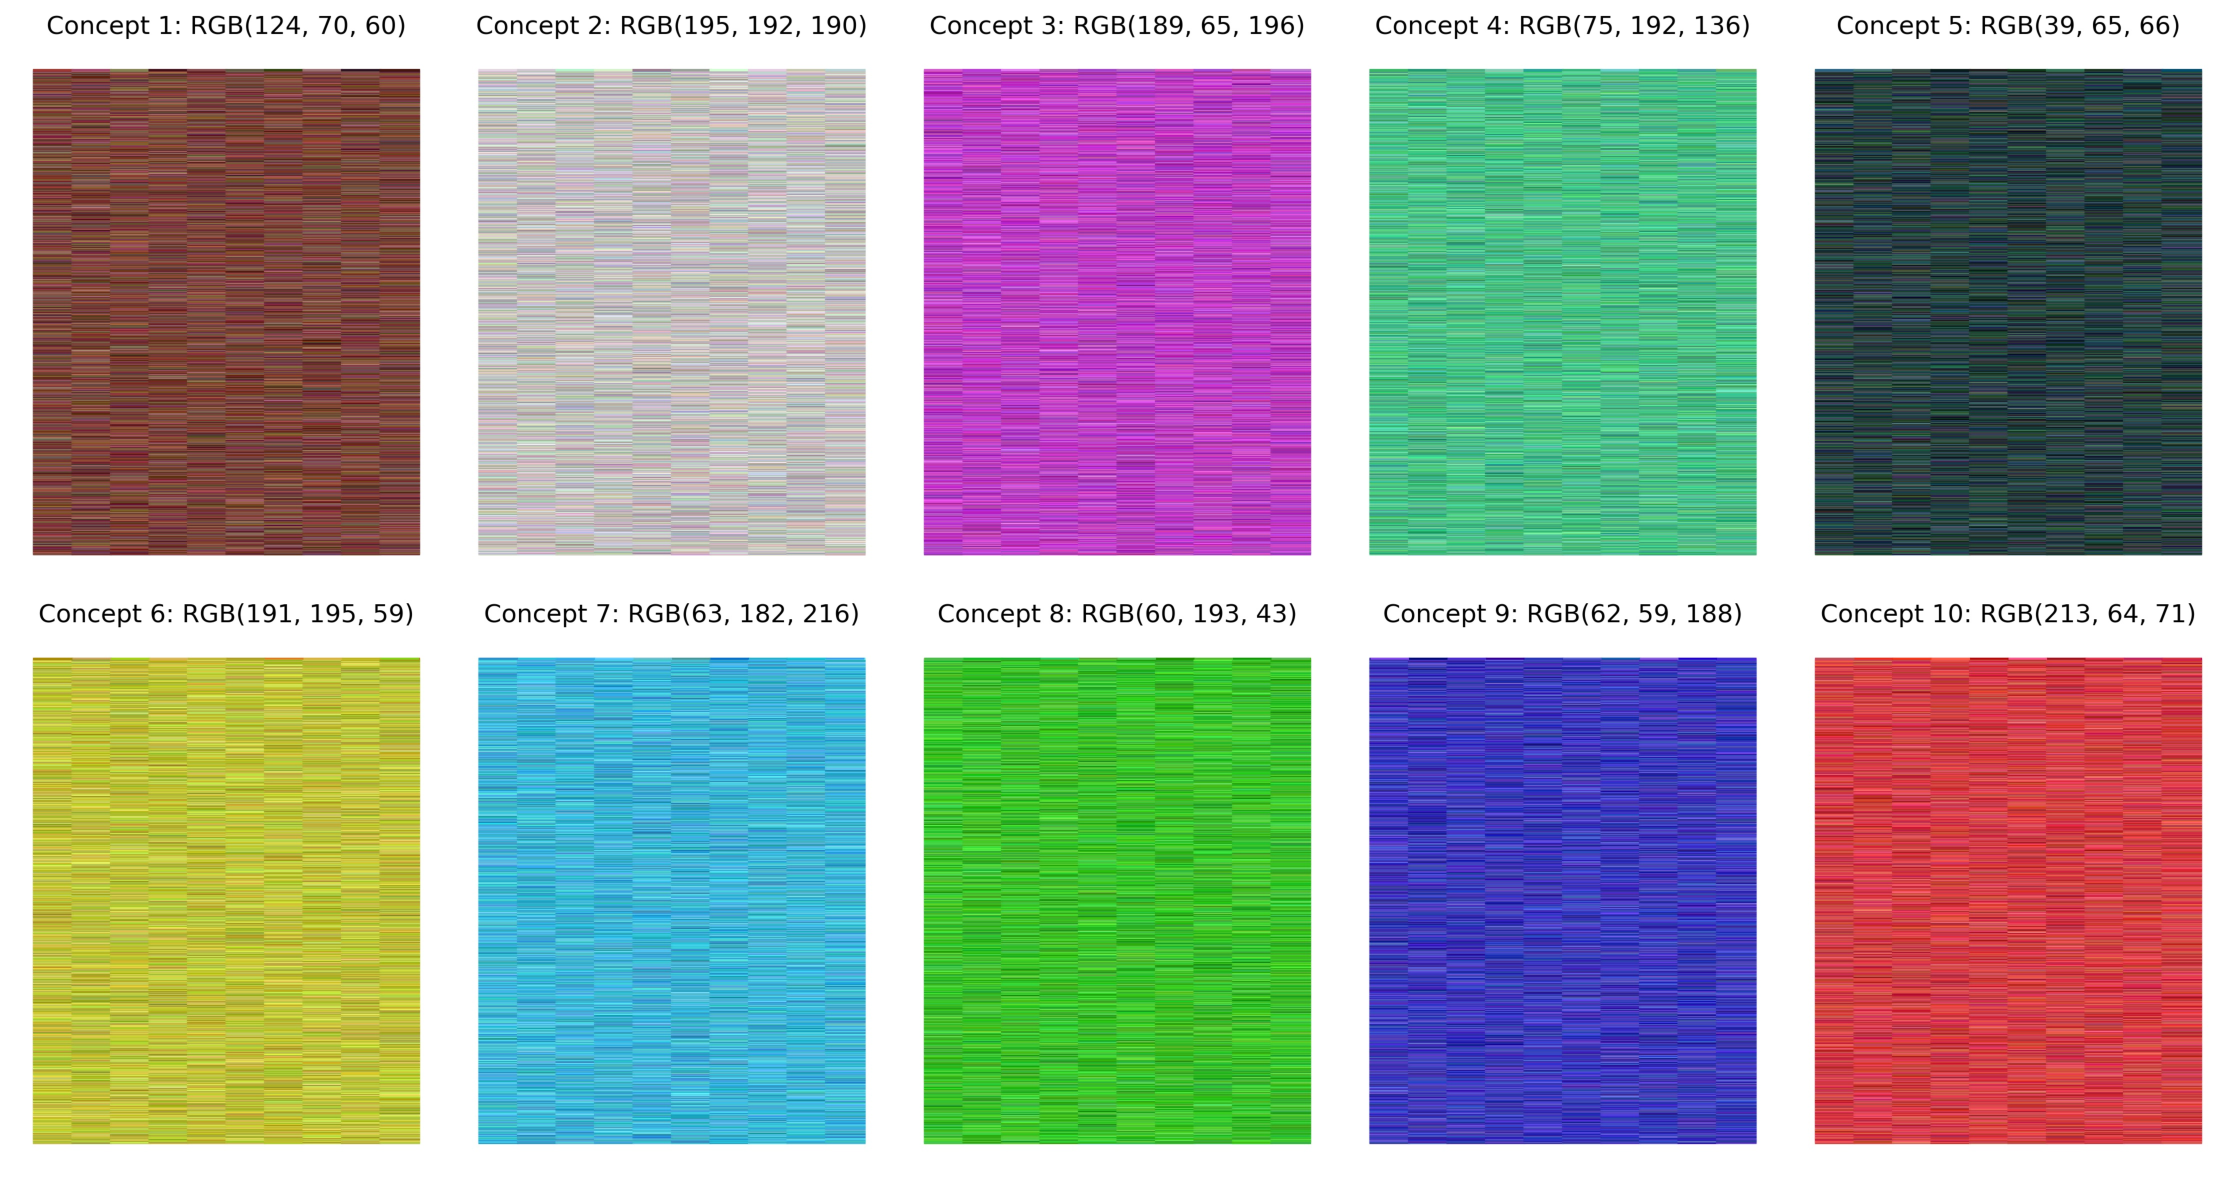
\includegraphics[width=\linewidth]{fig/color_varinace/1000.pdf}
    \caption{$\sigma^2 = 10^3$の場合の各色クラスの色の例}
    \label{fig:variance_1000}
\end{figure}

\begin{figure}[H]
    \centering
    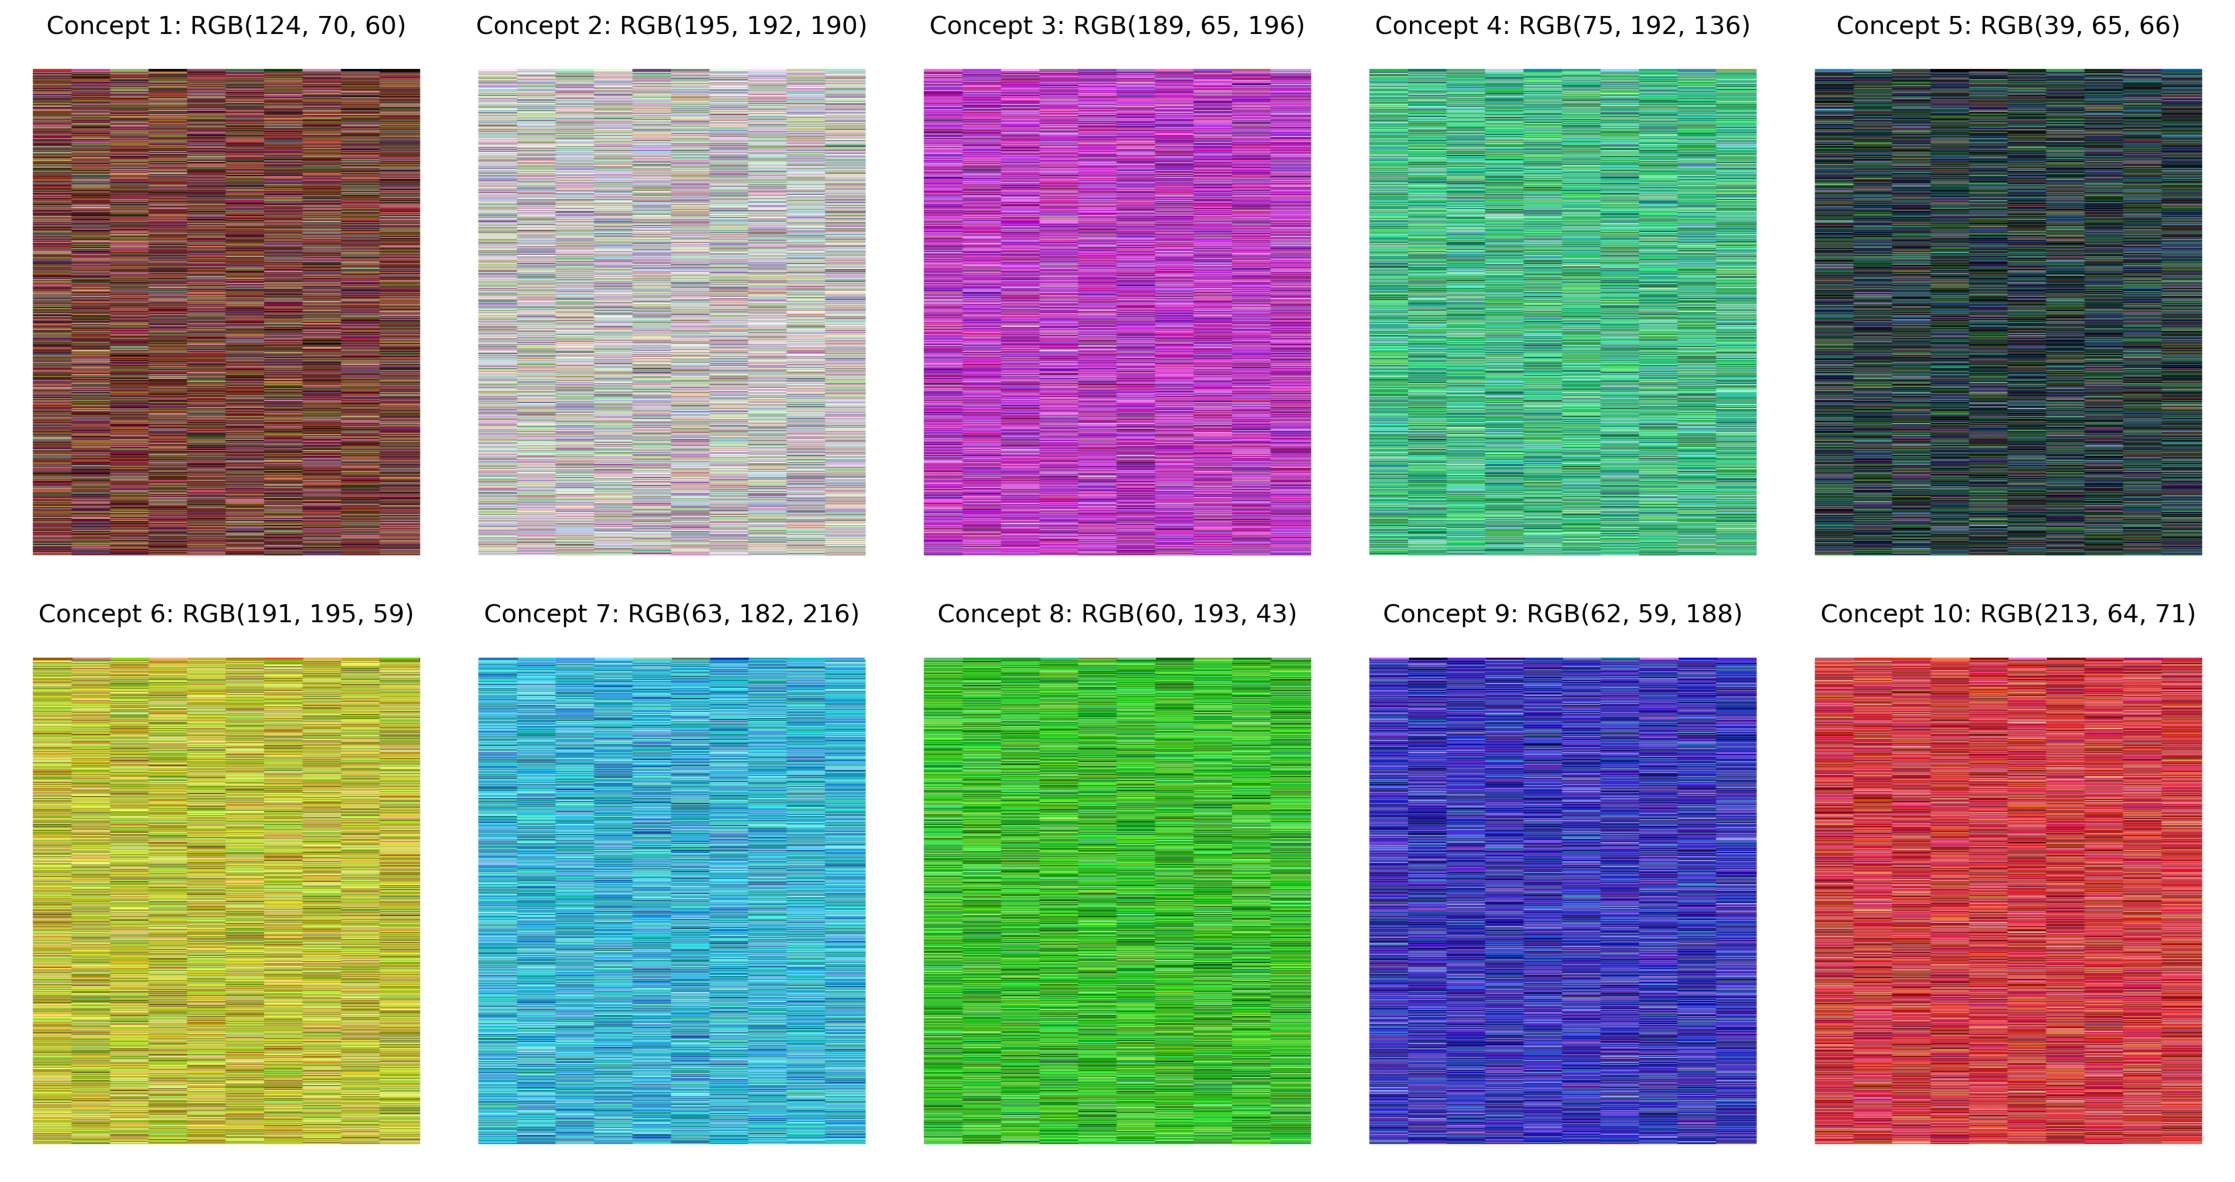
\includegraphics[width=\linewidth]{fig/color_varinace/3612.pdf}
    \caption{$\sigma^2 = 10^{3.5}$の場合の各色クラスの色の例}
    \label{fig:variance_3612}
\end{figure}

\begin{figure}[H]
    \centering
    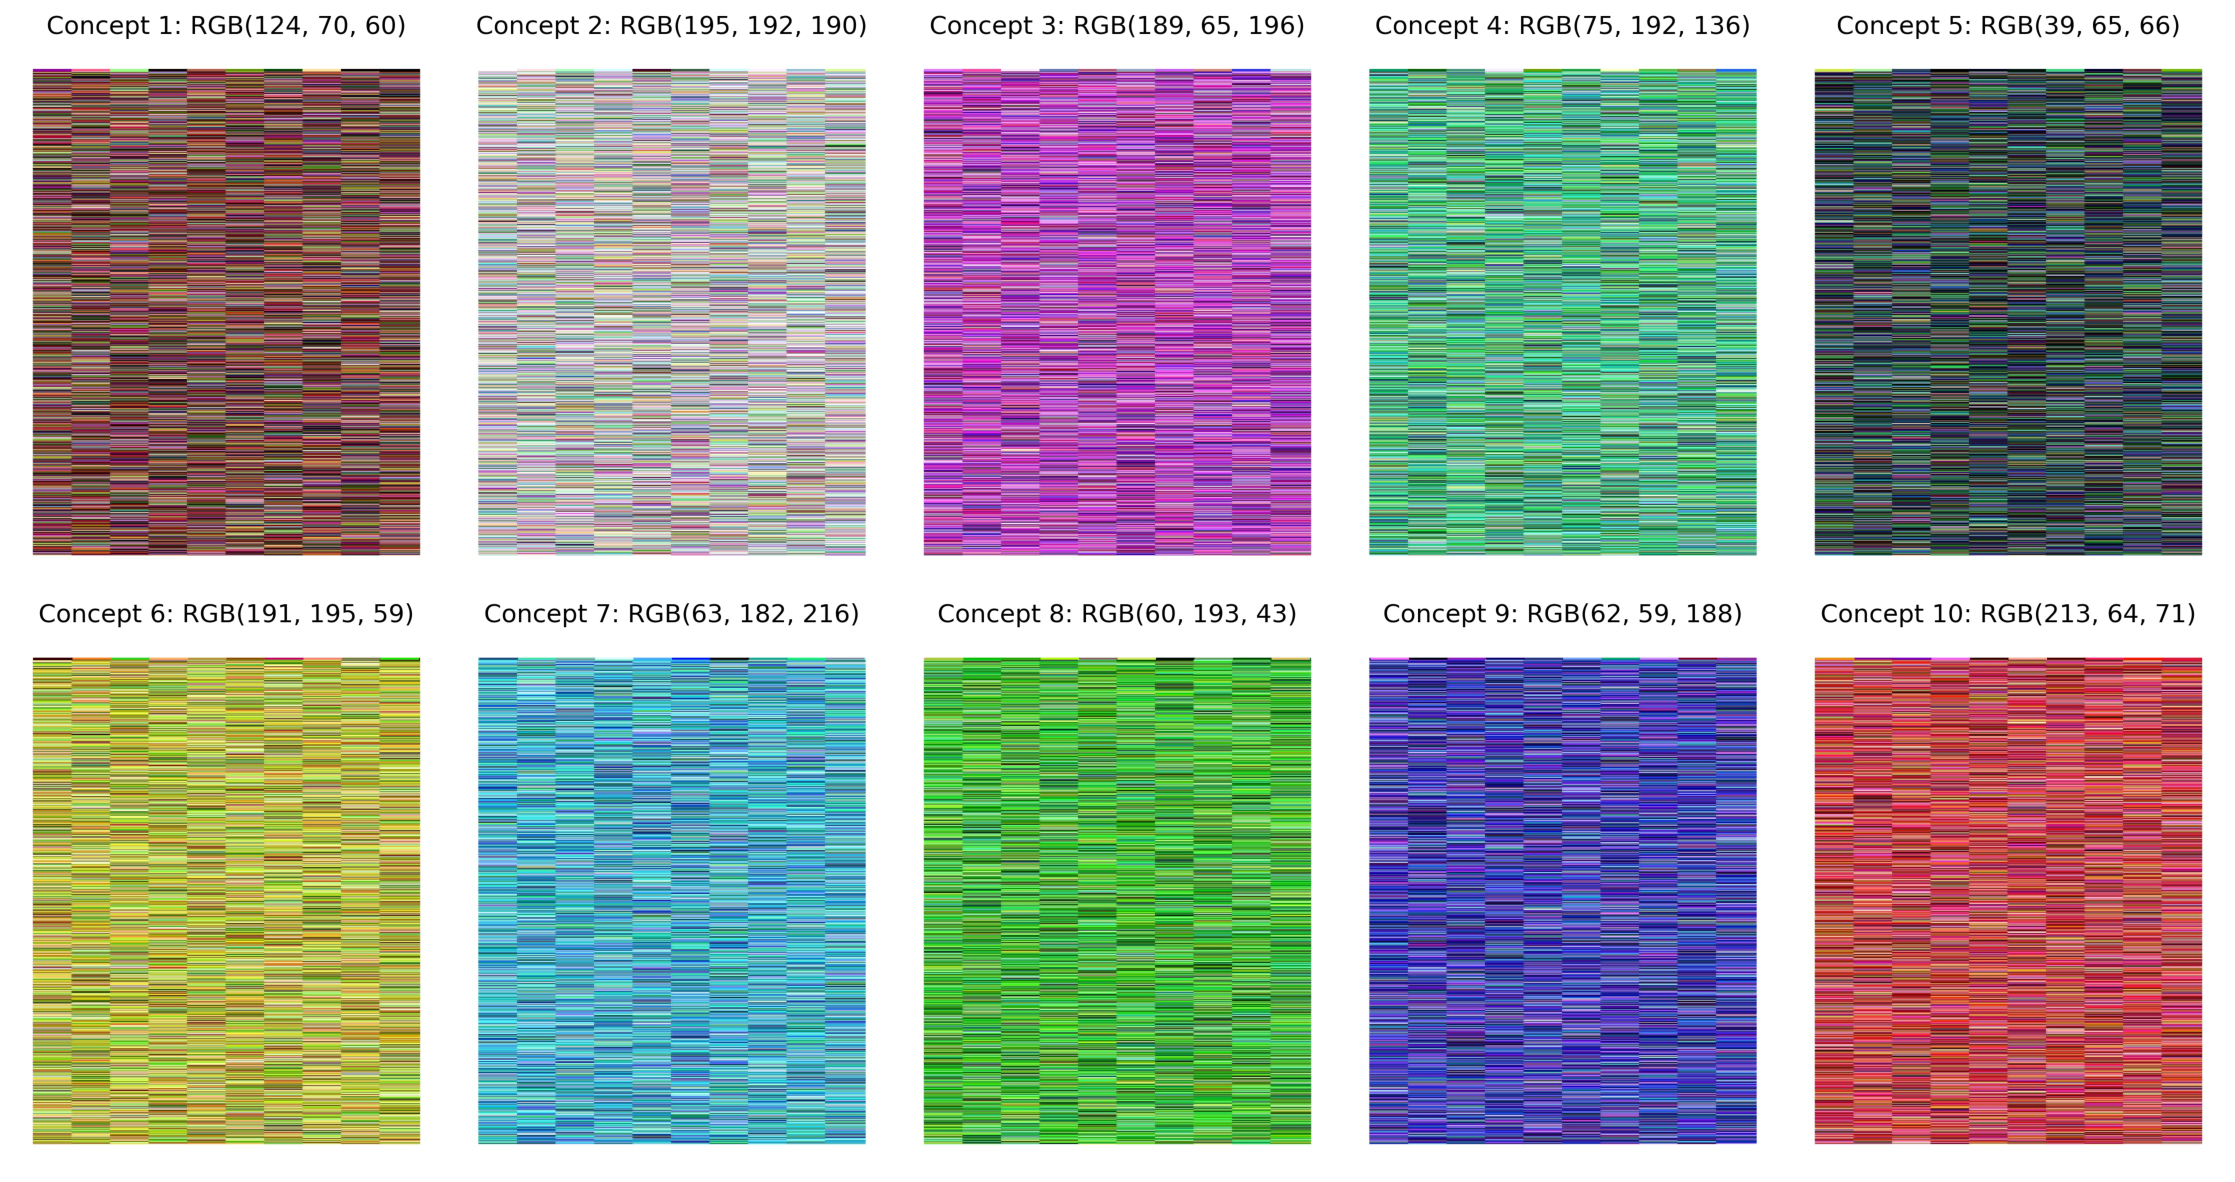
\includegraphics[width=\linewidth]{fig/color_varinace/10000.pdf}
    \caption{$\sigma^2 = 10^4$の場合の各色クラスの色の例}
    \label{fig:variance_10000}
\end{figure}

\begin{figure}[H]
    \centering
    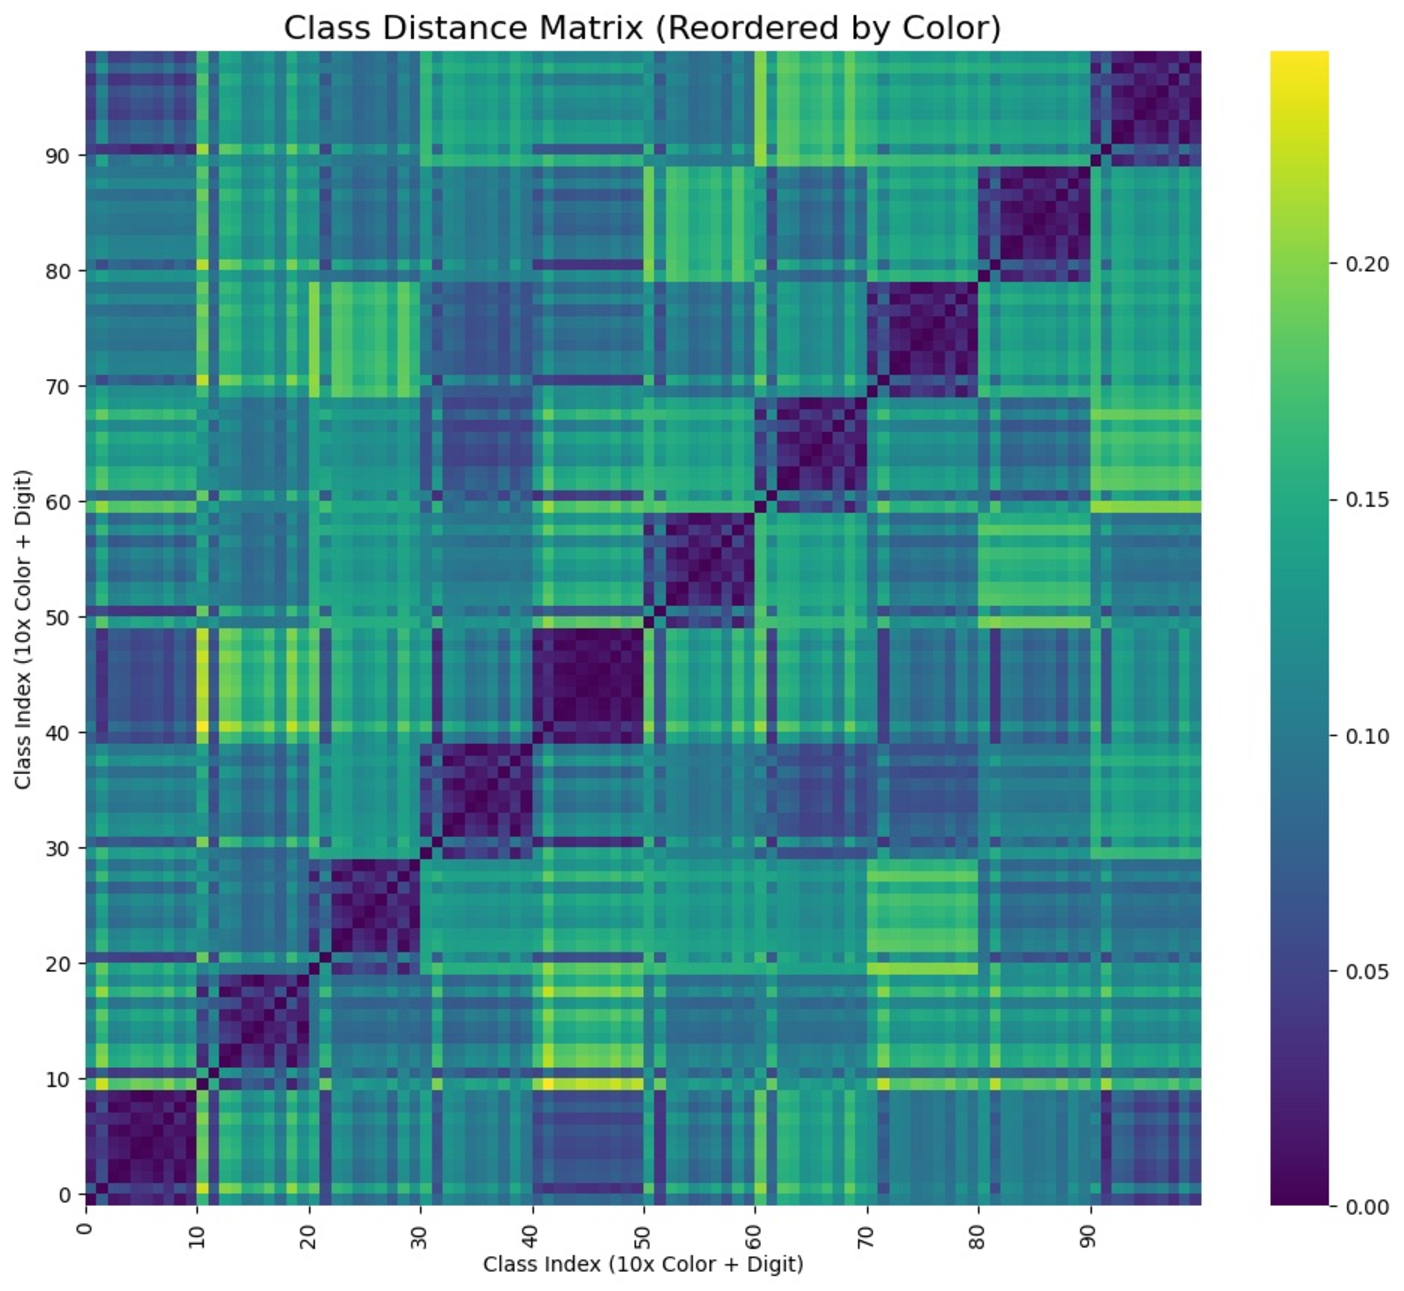
\includegraphics[width=\linewidth]{fig/distance_matrix_heatmap_by_color.pdf}
    \caption{100クラスのクラス間距離のヒートマップ(色,数字順)}
    \label{fig:distance_matrix_heatmap_by_color}
\end{figure}

\begin{figure}[H]
    \centering
    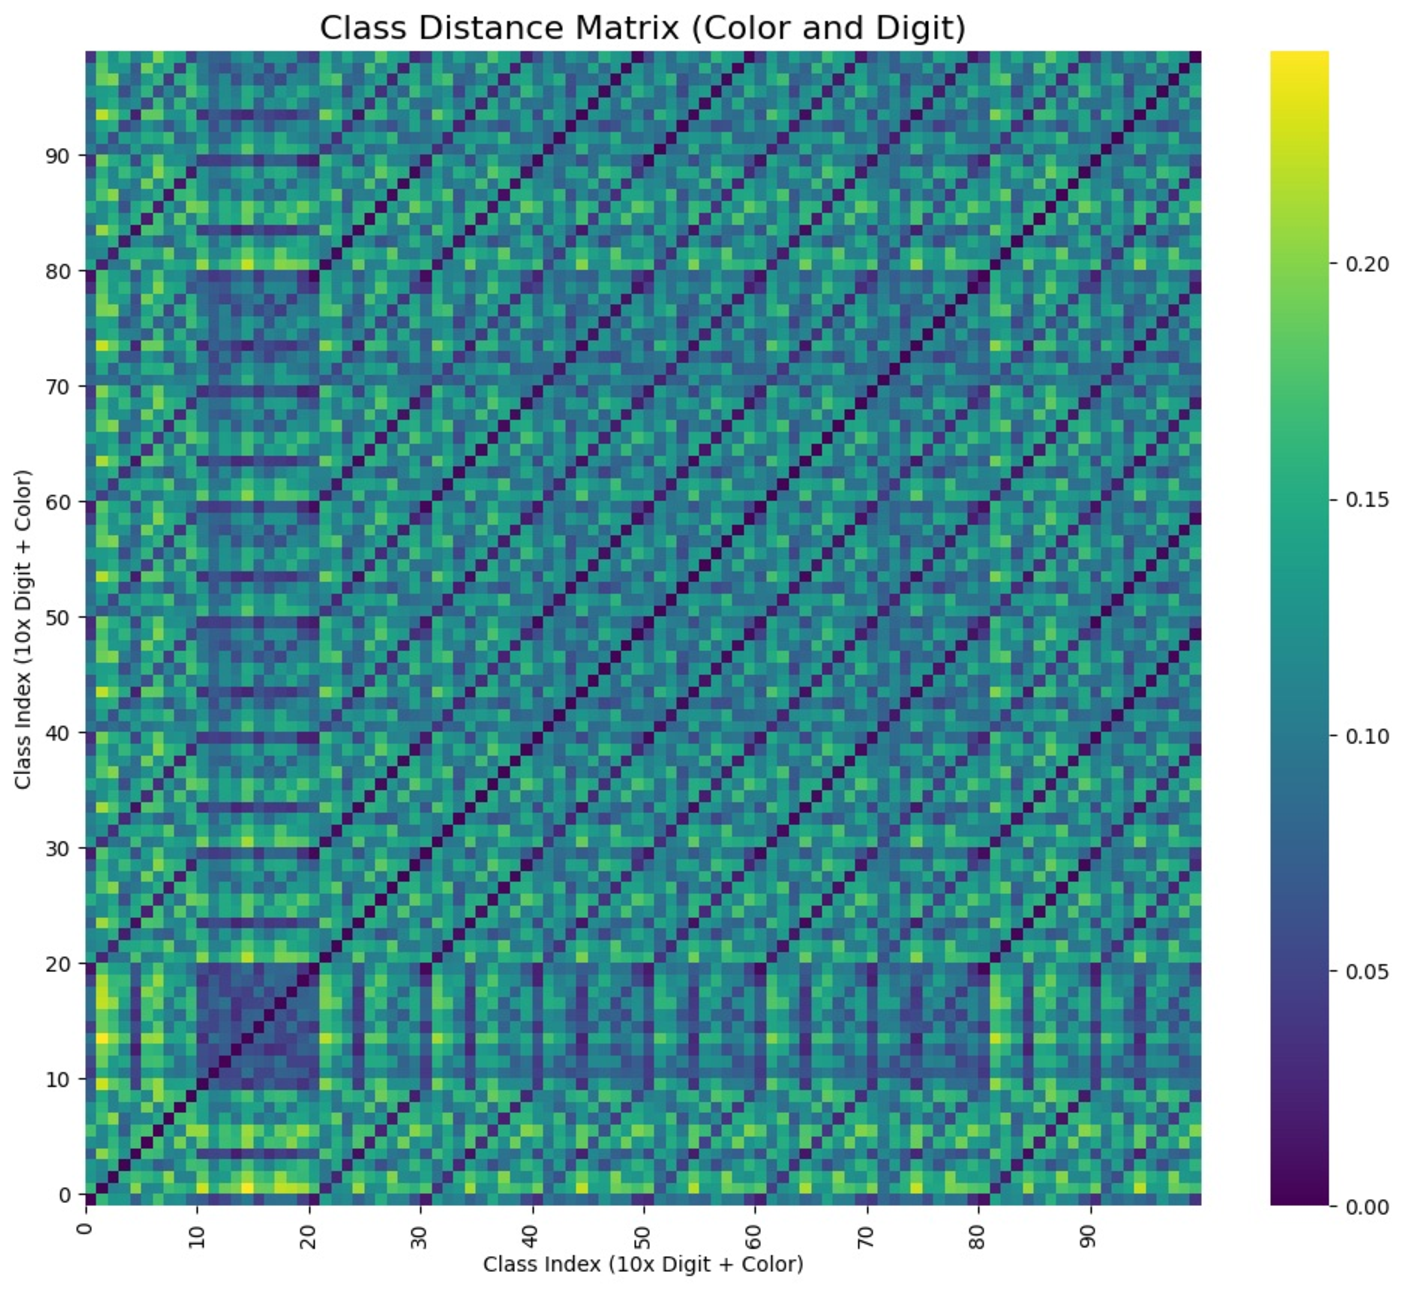
\includegraphics[width=\linewidth]{fig/distance_matrix_heatmap.pdf}
    \caption{100クラスのクラス間距離のヒートマップ(数字,色順)}
    \label{fig:distance_matrix_heatmap_by_digit}
\end{figure}

\begin{figure}[H]
    \centering
    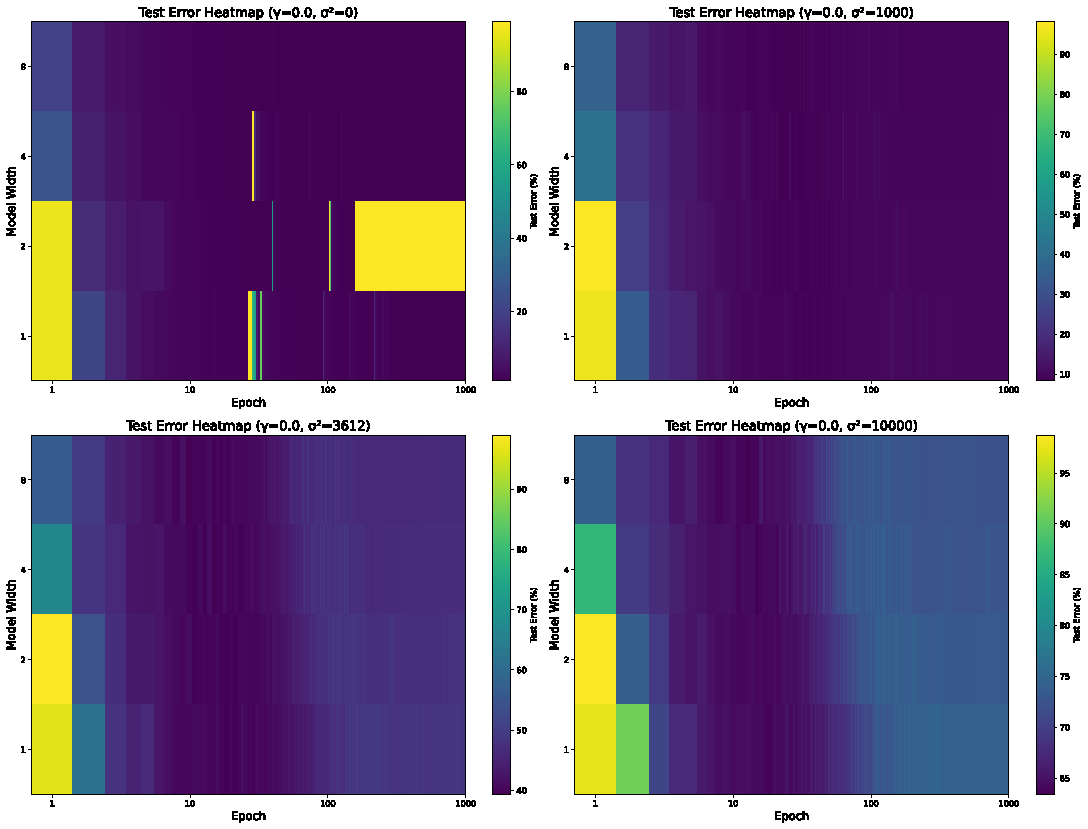
\includegraphics[width=\linewidth]{fig/heatmap_ln/ln0.pdf}
    \caption{$\gamma=0.0$のときのモデルのチャネル幅とエポック数によるテストエラー率のヒートマップ.
    }
    \label{fig:modelwidth_heatmap_0}
\end{figure}

\begin{figure}[H]
    \centering
    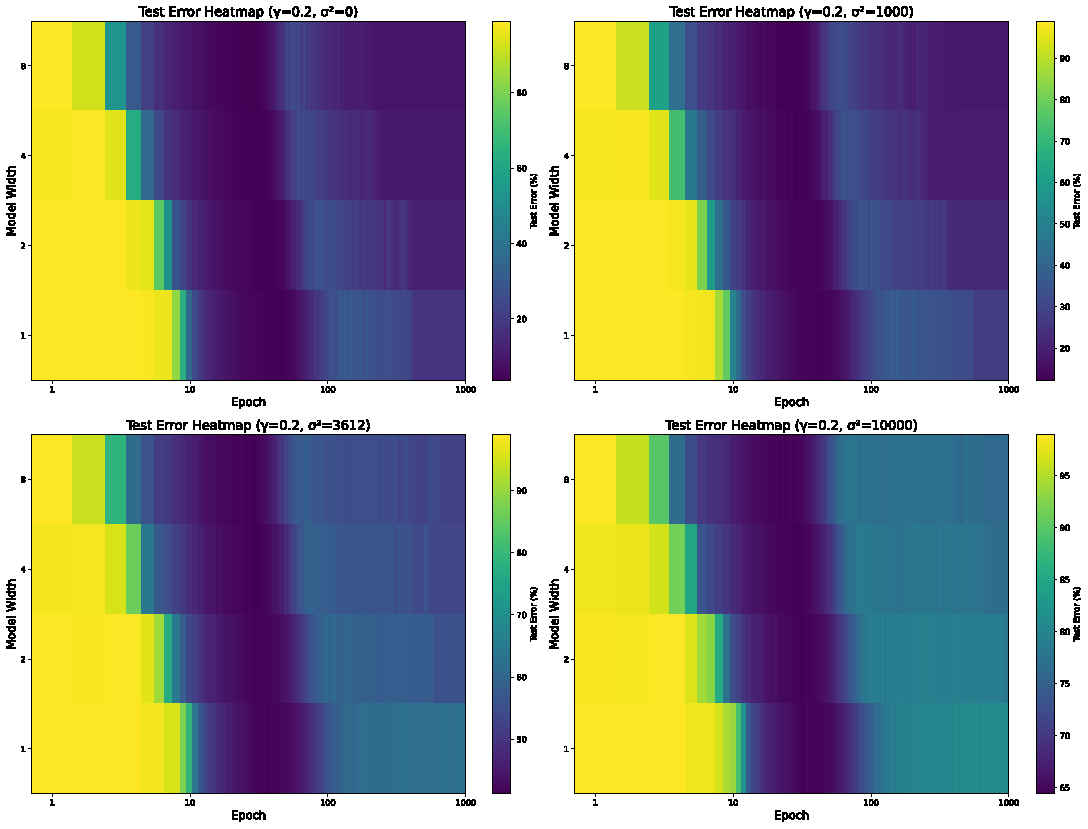
\includegraphics[width=\linewidth]{fig/heatmap_ln/ln0.2.pdf}
    \caption{$\gamma=0.2$のときのモデルのチャネル幅とエポック数によるテストエラー率のヒートマップ.}
    \label{fig:modelwidth_heatmap_0.2}
\end{figure}

\begin{figure}[H]
    \centering
    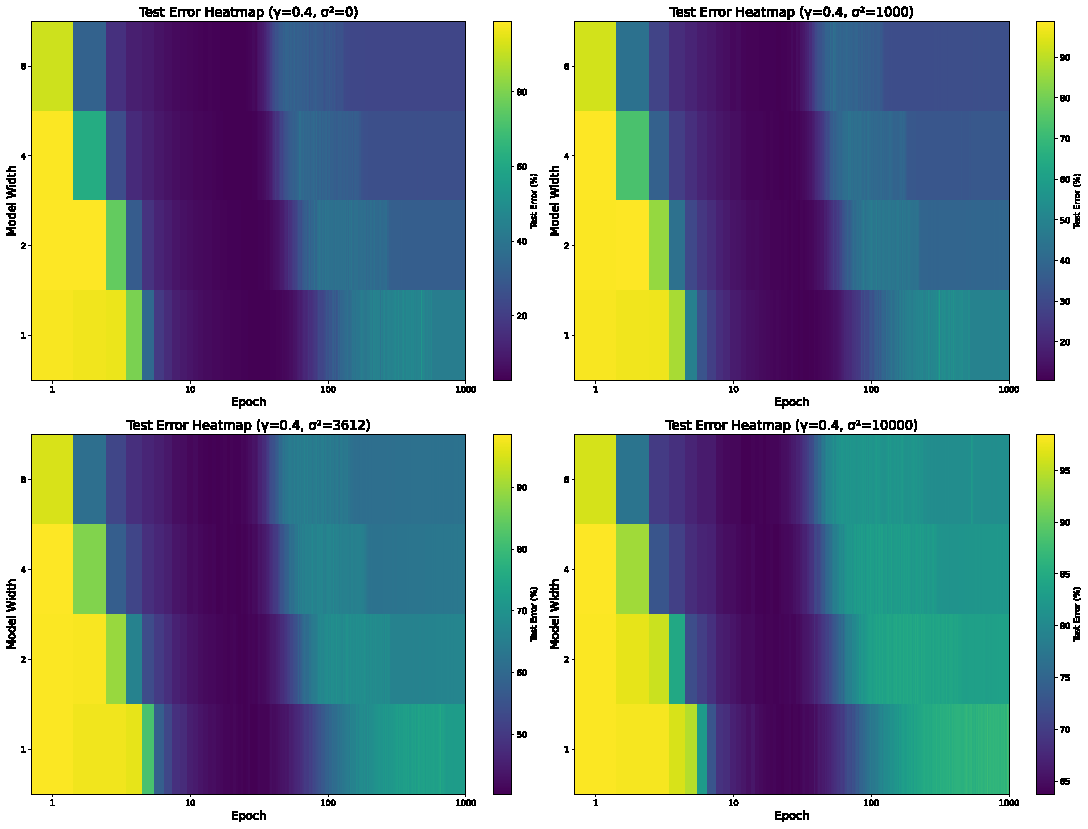
\includegraphics[width=\linewidth]{fig/heatmap_ln/ln0.4.pdf}
    \caption{$\gamma=0.4$のときのモデルのチャネル幅とエポック数によるテストエラー率のヒートマップ.}
    \label{fig:modelwidth_heatmap_0.4}
\end{figure}

\begin{figure}[H]
    \centering
    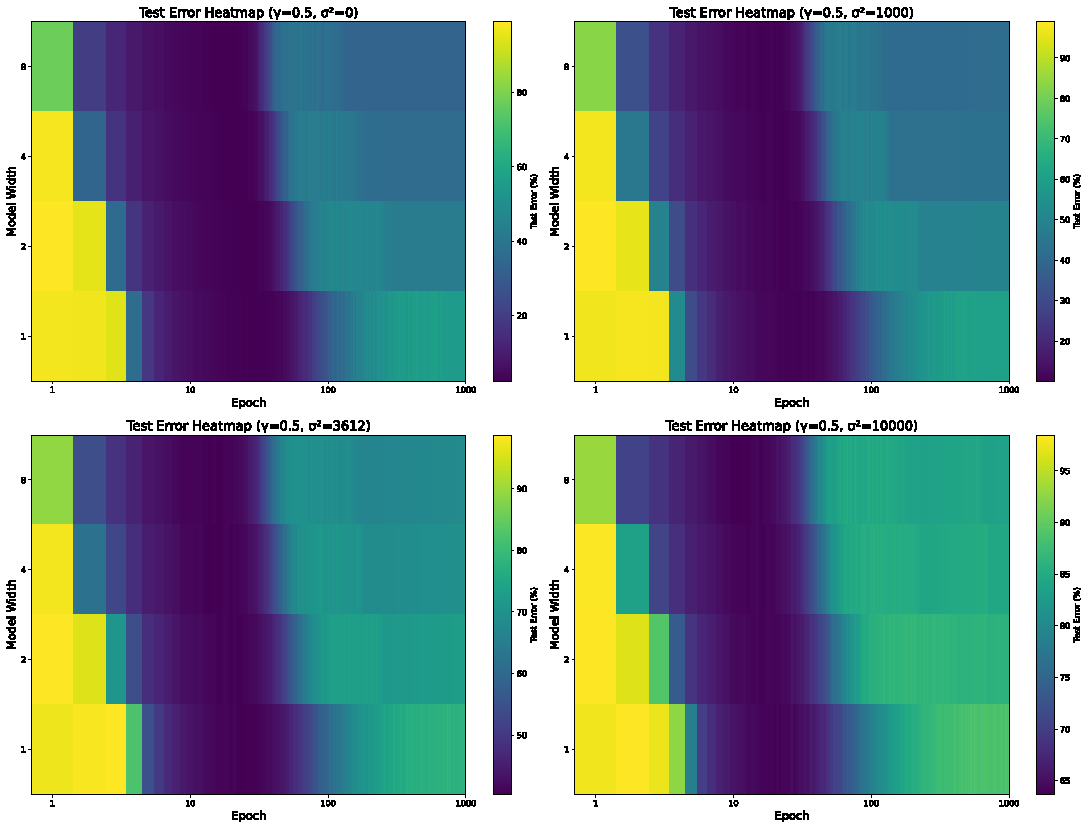
\includegraphics[width=\linewidth]{fig/heatmap_ln/ln0.5.pdf}
    \caption{$\gamma=0.5$のときのモデルのチャネル幅とエポック数によるテストエラー率のヒートマップ.}
    \label{fig:modelwidth_heatmap_0.5}
\end{figure}

\begin{figure}[H]
    \centering
    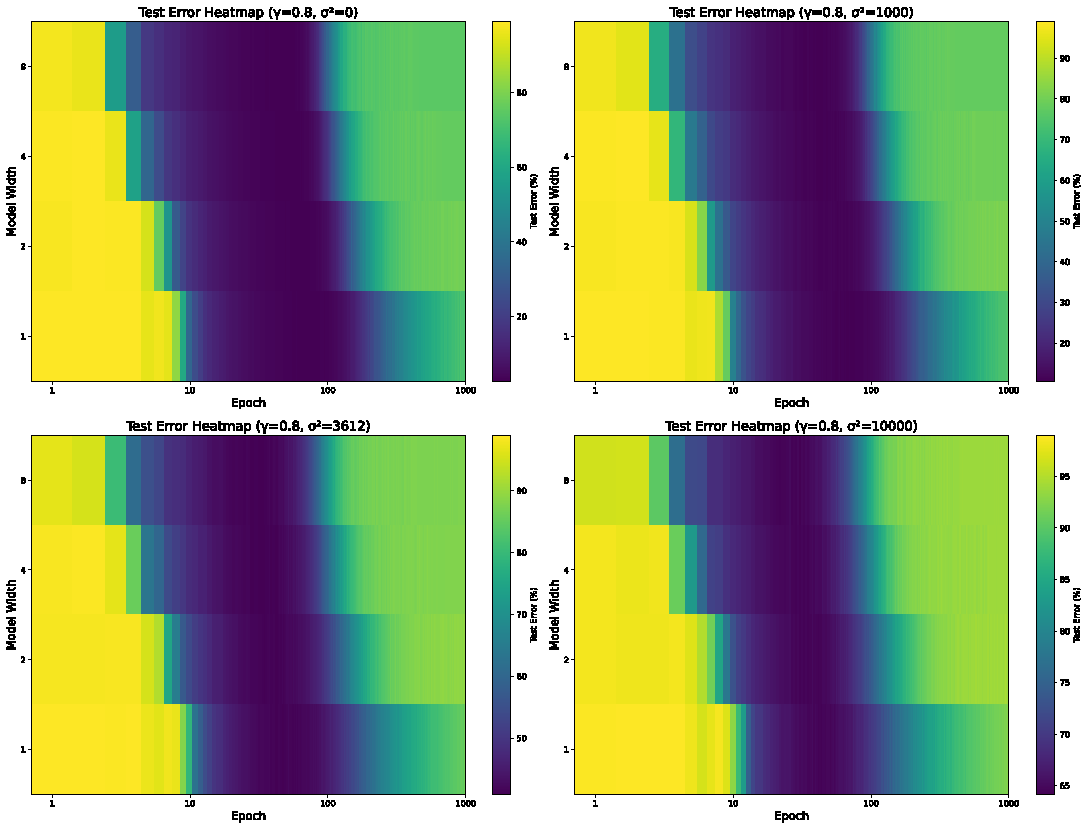
\includegraphics[width=\linewidth]{fig/heatmap_ln/ln0.8.pdf}
    \caption{$\gamma=0.8$のときのモデルのチャネル幅とエポック数によるテストエラー率のヒートマップ.}
    \label{fig:modelwidth_heatmap_0.8}
\end{figure}

\begin{figure}[H]
    \centering
    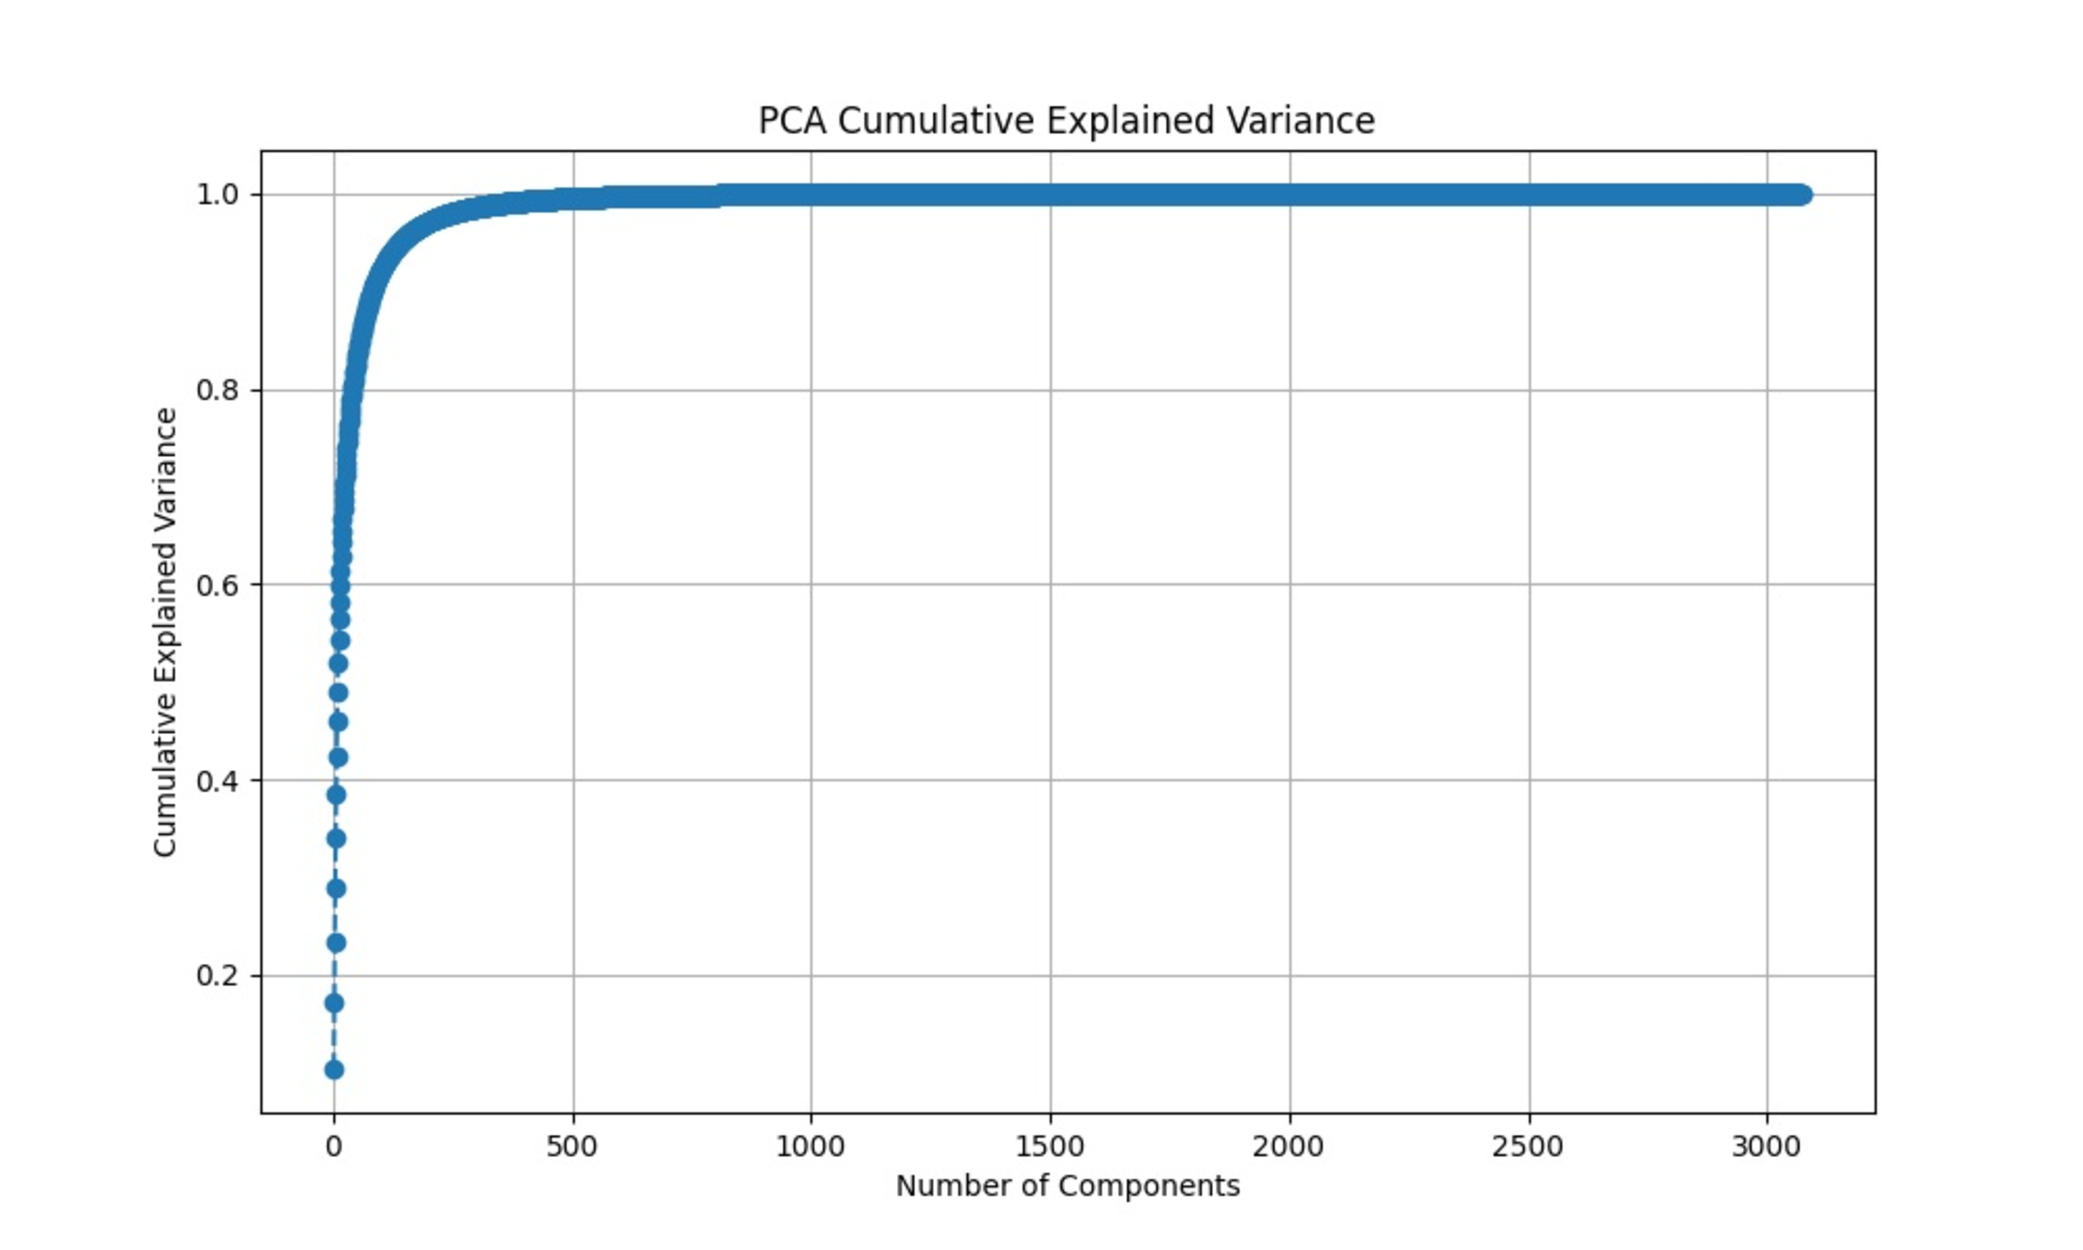
\includegraphics[width=\linewidth]{fig/kiyoritu_distribution_colored_EMNIST_Seed42_Var0_Corr0.5.pdf}
    \caption{Colored EMNISTデータセット($\sigma^2 = 0$)をPCAにかけたときの寄与率}
    \label{fig:modelwidth_heatmap_1}
\end{figure}

\begin{figure}[H]
    \centering
    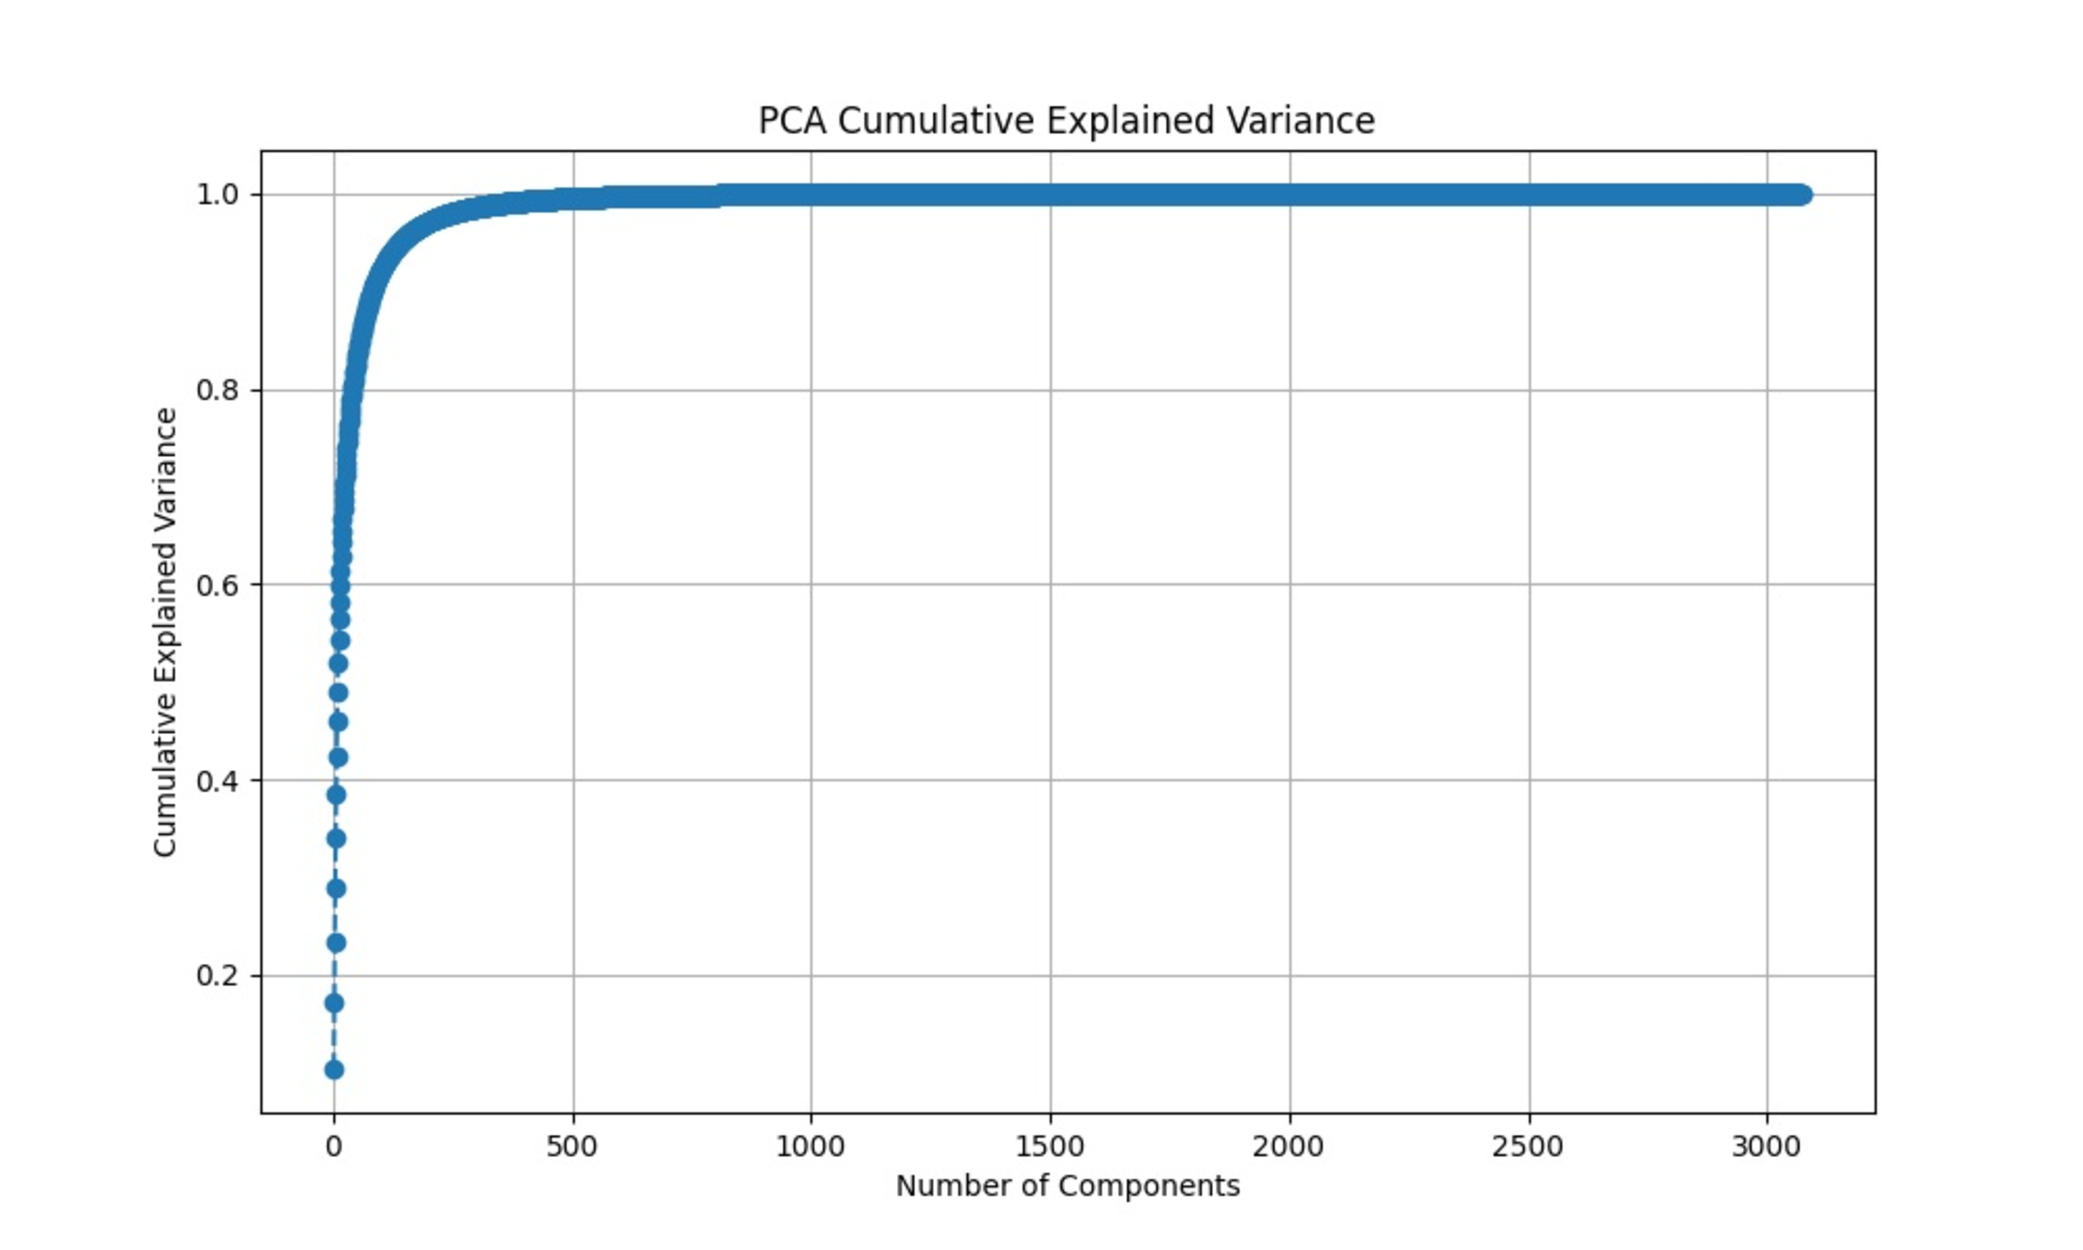
\includegraphics[width=\linewidth]{fig/kiyoritu_distribution_colored_EMNIST_Seed42_Var10000_Corr0.5.pdf}
    \caption{Colored EMNISTデータセット($\sigma^2 = 10^4$)をPCAにかけたときの寄与率}
    \label{fig:modelwidth_heatmap_1}
\end{figure}
